\documentclass[
	20pt% Default font size, values between 10pt-12pt are allowed
	%letterpaper, % Uncomment for US letter paper size
	%spanish, % Uncomment for Spanish
]{SUSTechHomework}

% Template-specific packages
\usepackage[american]{babel}
\usepackage{inputenc} % Required for inputting international characters
\usepackage[T1]{fontenc} % Output font encoding for international characters
\usepackage{mathpazo} % Use the Palatino font
\usepackage[scheme=plain]{ctex}
\usepackage{graphicx,subfigure} % Required for including images
\usepackage{booktabs} % Required for better horizontal rules in tables
\usepackage{listings} % Required for insertion of code
\usepackage[framed,numbered,autolinebreaks,useliterate]{mcode} %matlab代码
\usepackage{fontspec}
\usepackage{enumerate} % To modify the enumerate environment
\usepackage{amsmath}
\usepackage{amssymb}
\usepackage{mathptmx}
\usepackage{bm}
%----------------------------------------------------------------------------------------
\setmainfont{Times New Roman}

% 代码模板
\lstdefinestyle{mystyle}{
    basicstyle=\ttfamily\footnotesize,
    breakatwhitespace=false,         
    breaklines=true,                 
    keepspaces=true,                 
    numbers=left,                    
    numbersep=5pt,                  
    showspaces=false,                
    showstringspaces=false,
    tabsize=4
}
\lstset{style=mystyle}
% 使用方法:\lstinputlisting[language=Python]{code/a2.py}
%----------------------------------------------------------------------------------------
%	ASSIGNMENT INFORMATION
%----------------------------------------------------------------------------------------

\title{Final-Project} % Assignment title
\author{Fudong Deng} % Student name and ID
\sid{12132389}
\date{June 9 2022} % Due date
% \centering
\includegraphics[scale=0.75]{img/logo.png}
%\institute{SOUTHERN UNIVERSITY\\OF SCIENCE AND TECHNOLOGY} % Institute or school name
\coursecode{MAE5032}
\coursename{High Performace Computing} % Course or class name
% \professor{Prof. Liu } % Professor or teacher in charge of the assignment

% \makeatletter
% \renewcommand{\section}{\@startsection{section}{1}{0mm}
% {-\baselineskip}{0.5\baselineskip}{\bf\leftline}}
% \makeatother

\begin{document}
\maketitle 
\large 
%----------------------------------------------------------------------------------------
\section{公式推导以及稳定性分析}
\qquad 一维传热方程如下:
\begin{equation*}
    \rho c \frac{\partial u}{\partial t} - \kappa \frac{\partial^2 u}{\partial x^2} = \sin(l \pi x)
\end{equation*}
\qquad 边界条件为:
$$
\begin{aligned}
u(0,t) &= u(1,t) = 0\\
u|_{t=0} &= e^x
\end{aligned}
$$
\qquad 则可将传热方程改写为:$\frac{\partial u}{\partial t} - \frac{\kappa}{\rho c}\frac{\partial^2 u}{\partial x^2} = \frac{1}{\rho c}\sin(l \pi x)$
\subsection{显示格式(Adams-Bashforth)}
\qquad 差分格式为:
$$
\left\{ 
    \begin{array}{c}
        \begin{aligned}
        \frac{\partial u}{\partial t} &= \frac{u^{n+1}_j-u^n_j}{\Delta t}\\
        \frac{\partial^2 u}{\partial x^2} &= \frac{u^n_{j+1}-2u^n_j+u^n_{j-1}}{\Delta x^2}
        \end{aligned}
    \end{array}
\right.
$$

$$
\begin{aligned}
\therefore \frac{u^{n+1}_j-u^n_j}{\Delta t} &= \frac{\kappa}{\rho c} \frac{u^n_{j+1}-2u^n_j+u^n_{j-1}}{\Delta x^2} + \frac{1}{\rho c}\sin(l \pi j \Delta x) \\
\implies u^{n+1}_j &= u^n_j + \frac{\kappa \Delta t}{\rho c \Delta x^2} (u^n_{j+1}-2u^n_j+u^n_{j-1})+ \frac{\Delta t}{\rho c}\sin(l \pi j \Delta x)\\
\implies u^{n+1}_j &= \frac{\kappa \Delta t}{\rho c \Delta x^2} u^n_{j+1} + (1-\frac{2 \kappa \Delta t}{\rho c \Delta x^2}) u^n_j + \frac{\kappa \Delta t}{\rho c \Delta x^2}u^n_{j-1} + \frac{\Delta t}{\rho c}\sin(l \pi j \Delta x)\\
make  \frac{\kappa}{\rho c} &= \alpha, \frac{\alpha \Delta t}{\Delta x^2} = \beta = \frac{\kappa \Delta t}{\rho c \Delta x^2}\\
\implies u^{n+1}_j &= \beta u^n_{j+1} + (1-2\beta) u^n_j + \beta u^n_{j-1} + \frac{\Delta t}{\rho c}\sin(l \pi j \Delta x)\\
\end{aligned}
$$

$$
\begin{pmatrix}
    u^{n+1}_1 - \alpha \Delta t \sin(l \pi \Delta x) \\
    u^{n+1}_2 - \alpha \Delta t \sin(l \pi 2 \Delta x)\\
    \vdots\\
    u^{n+1}_{n-2} - \alpha \Delta t \sin(l \pi (n-2) \Delta x)\\
    u^{n+1}_{n-1} - \alpha \Delta t \sin(l \pi (n-1) \Delta x)\\
\end{pmatrix}=
\begin{pmatrix}
    1-2 \beta & \beta & 0 & 0 & \cdots & 0 & 0 & 0\\
    \beta & 1-2 \beta & \beta & 0 & \cdots & 0 & 0 & 0\\
    0 & \beta & 1-2 \beta & \beta & \cdots & 0 & 0 & 0\\
    \vdots & \vdots & \vdots & \vdots & \ddots & \vdots & \vdots & \vdots\\
    0 & 0 & 0 & 0 & \cdots & 0 & \beta & 1-2\beta \\
\end{pmatrix}*
\begin{pmatrix}
    u^{n}_1  \\
    u^{n}_2 \\
    \vdots\\
    u^{n}_{n-2}\\
    u^{n}_{n-1}\\
\end{pmatrix}
$$
\subsubsection{稳定性分析}
\qquad 由von-Neumann稳定性分析可得:

$$
\begin{aligned}
\delta u_j^{n+1} &=\beta \delta u_{j-1}^{n} + (1-2\beta)\delta u_j^{n} + \beta \delta u_{j+1}^{n}\\
\because \delta u_j^n &\backsim e^{\sigma n \Delta t} \cdot e^{i(k \cdot j \Delta x)}\\
\therefore e^{\sigma \Delta t} &= \beta e^{i k \Delta x} + (1-2\beta) + \beta e^{-i k \Delta x}\\
&= (1-2\beta) + \beta (e^{i k \Delta x} + e^{-i k \Delta x})\\
\end{aligned}
$$

由$\lvert e^{\sigma \Delta t} \rvert < 1 \implies \lvert (1-2\beta) + \beta \cos(k \Delta x)) \rvert < 1 \implies \lvert 1-4\beta \rvert < 1 \implies 0 \leq \beta \leq 0.5$

\subsection{隐式格式(Crank-Nicolson)}
\qquad 差分格式为:

$$
\left\{ 
    \begin{array}{c}
        \begin{aligned}
        \frac{\partial u}{\partial t} &= \frac{u^{n+1}_j-u^n_j}{\Delta t}\\
        \frac{\partial^2 u}{\partial x^2} &= \frac{u^{n+1}_{j+1}-2u^{n+1}_j+u^{n+1}_{j-1}}{\Delta x^2}
        \end{aligned}
    \end{array}
\right.
$$

$$
\begin{aligned}
\therefore \frac{u^{n+1}_j-u^n_j}{\Delta t} &= \frac{\kappa}{\rho c} \frac{u^{n+1}_{j+1}-2u^{n+1}_j+u^{n+1}_{j-1}}{\Delta x^2} + \frac{1}{\rho c}\sin(l \pi j \Delta x)\\
make  \frac{\kappa}{\rho c} &= \alpha, \frac{\alpha \Delta t}{\Delta x^2} = \beta = \frac{\kappa \Delta t}{\rho c \Delta x^2}\\
\end{aligned}
$$

$$
\begin{aligned}
\implies -\beta u^{n+1}_{j-1} + (1+2\beta)u^{n+1}_j - \beta u^{n+1}_{j+1} = u^n_j + \frac{\Delta t}{\rho c} \sin(l \pi j \Delta x)
\end{aligned}
$$

\qquad 解的格式为:

$$
\begin{pmatrix}
    1+2 \beta & -\beta & 0 & \cdots & 0 & 0 & 0\\
    -\beta & 1+2 \beta & -\beta & \cdots & 0 & 0 & 0\\
    \vdots & \vdots & \vdots & \ddots & \vdots & \vdots & \vdots\\
    0 & 0 & 0 & \cdots & -\beta & 1+2\beta & -\beta\\
    0 & 0 & 0 & \cdots & 0 & -\beta & 1+2\beta\\
\end{pmatrix}
\begin{pmatrix}
    u^{n+1}_1  \\
    u^{n+1}_2 \\
    \vdots\\
    u^{n+1}_{n-2}\\
    u^{n+1}_{n-1}\\
\end{pmatrix}=
\begin{pmatrix}
    u^{n}_1 + \frac{\Delta t}{\rho c} \sin(l \pi \Delta x) \\
    u^{n}_2 + \frac{\Delta t}{\rho c} \sin(l \pi 2 \Delta x)\\
    \vdots\\
    u^{n}_{n-2} + \frac{\Delta t}{\rho c} \sin(l \pi (n-2) \Delta x)\\
    u^{n}_{n-1} + \frac{\Delta t}{\rho c} \sin(l \pi (n-1) \Delta x)\\
\end{pmatrix}
$$
\subsubsection{稳定性分析}

由von-Neumann稳定性分析可得:
$$
\begin{aligned}
-\beta \delta u_{j-1}^{n+1} &+ (1+2\beta)\delta u_j^{n+1} - \beta \delta u_{j+1}^{n+1} = \delta u_j^n\\
\because \delta u_j^n &\backsim e^{\sigma n \Delta t} \cdot e^{i(k \cdot j \Delta x)}\\
\therefore -\beta e^{\sigma \Delta t} \cdot e^{-ik\Delta x} &+ (1+2\beta)e^{\sigma \Delta t} - \beta e^{\sigma \Delta t} \cdot e^{i k \Delta x} = 1\\
e^{\sigma n \Delta t}(\beta e^{i k \Delta t} &+ \beta e^{-i k \Delta t} - (1+2\beta)) = -1\\
\implies e^{\sigma n \Delta t} &= \frac{-1}{\beta e^{i k \Delta t} + \beta e^{-i k \Delta t} - (1+2\beta)}\\
\end{aligned}
$$

由 $\lvert e^{\sigma \Delta t} \rvert < 1 \implies \lvert \frac{1}{1 + 2\beta (1-\cos(k \Delta x))} \rvert < 1 \implies \beta$ 可以为任何值

\section{结果显示}
\subsection{结果验证}
\qquad 一维传热方程解析解为:$\frac{\sin(l \pi x)}{\pi^2} - \frac{\sin(l \pi)}{\pi^2} $,在$l=1$的情况下,解析解为:$\frac{\sin(\pi x)}{\pi^2}$。

\qquad 显式格式情况下,设置网格数量$n=100$,$CFL=0.2$,隐式格式为设置网格数$n=100,CFL=1$的情况下,解析解以及显式格式与隐式格式的解如下图所示:
\begin{figure}[hb]
    \centering
    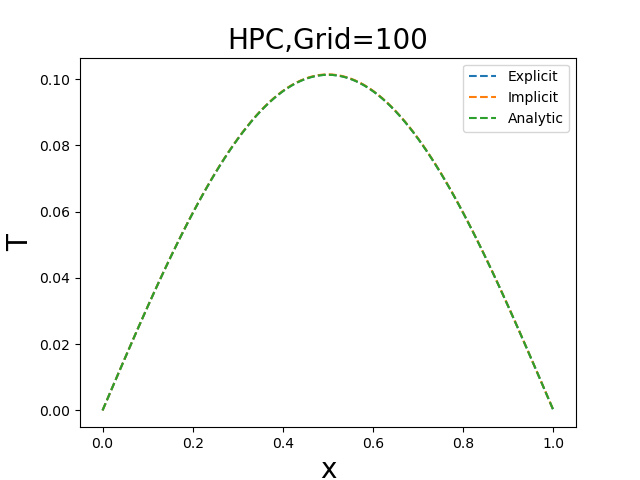
\includegraphics[width=300pt]{img/n=100.png}
    \caption{结果验证}
    \label{fig:figure1}
\end{figure}

\qquad 可以得到,显式解与隐式解与解析解基本重合,验证了显式格式以及隐式格式的准确性。但是由于显式格式稳定性条件的影响,当显式格式网格数增大时,时间步长需要随之减小从而使得计算量大大增加。而隐式格式的稳定性比较好,所以增加网格数量时,时间不长不用减少而计算量比显式要小,所用时间也比显式格式的要少。
\clearpage
\subsection{并行性展示}
\qquad  显式格式下,展示程序的并行强可扩展性,在网格数较少的时候,CPU核数增加,导致程序运行时间也增加,预估为网格数较少,各个CPU之间通信时间为主要部分,网格数$n=5000,CFL=0.5$,得到在不同核数量下运行时间如图所示:
\begin{figure}[h]
    \centering
    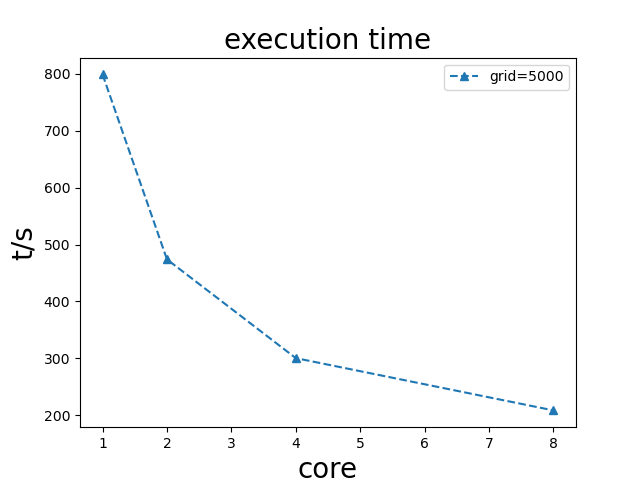
\includegraphics[width=300pt]{img/execution time.png}
    \caption{不同核数相同网格的运行时间}
    \label{fig:my_label}
\end{figure}

\qquad 显式格式下,展示程序的并行弱可扩展性,不同核数但是$grid/core=1000$,以及$dt=1e-8$,得到在不同核数量下运行时间如图所示:
\begin{figure}[h]
    \centering
    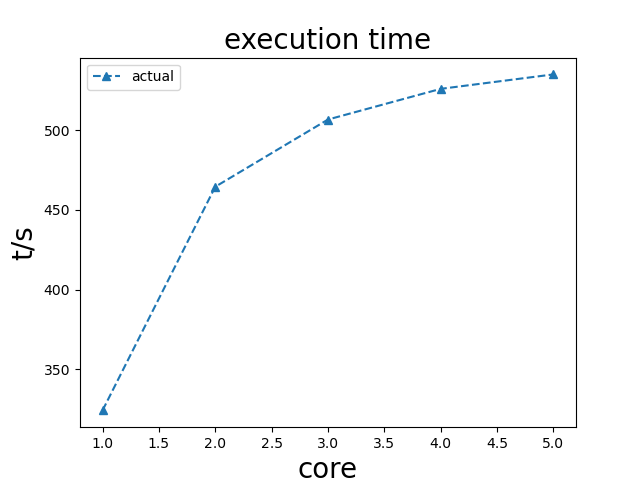
\includegraphics[width=300pt]{img/execution.png}
    \caption{不同核数不同网格的运行时间}
    \label{fig:my_label}
\end{figure}

\clearpage
\qquad  隐式格式下,展示程序的并行强可扩展性,在网格数较少的时候,CPU核数增加,导致程序运行时间也增加,预估为网格数较少,各个CPU之间通信时间为主要部分,网格数$n=5000,dt=0.0001$,得到在不同核数量下运行时间如图所示:
\begin{figure}[h]
    \centering
    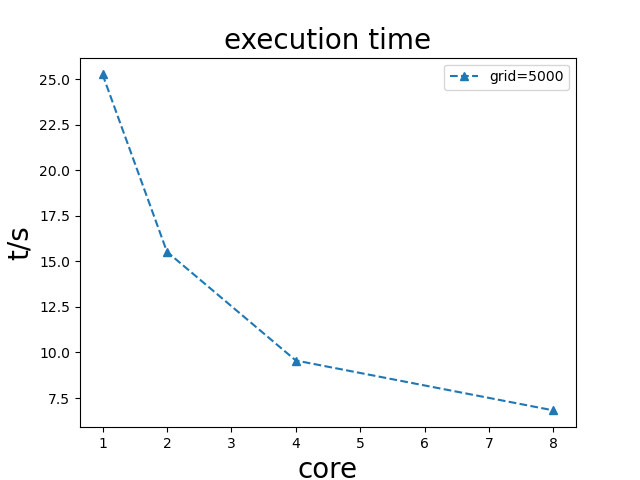
\includegraphics[width=300pt]{img/Implicit_Exec.png}
    \caption{不同核数相同网格的运行时间}
    \label{fig:my_label}
\end{figure}

\qquad 隐式格式下,展示程序的并行弱可扩展性,不同核数但是$grid/core=1000$,以及$dt=1e-8$,得到在不同核数量下运行时间如图所示:
\begin{figure}[h]
    \centering
    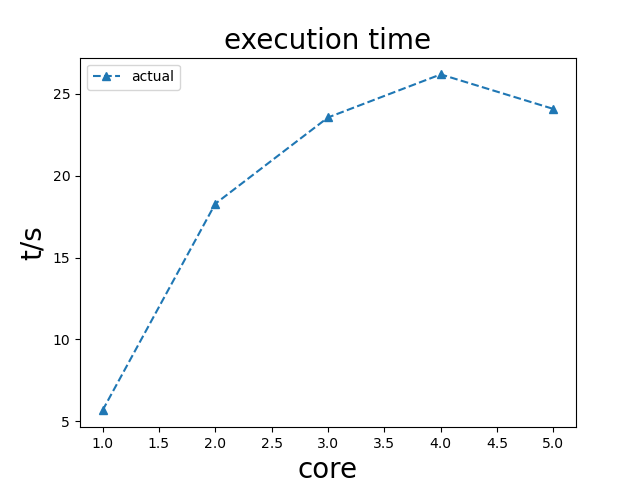
\includegraphics[width=300pt]{img/Implicit_E.png}
    \caption{不同核数不同网格的运行时间}
    \label{fig:my_label}
\end{figure}
\clearpage
\subsection{误差分析}
\qquad 显式格式情况下,固定$dt=0.000002$,改变网格数量$n$分别取$100, 200, 300, 400$得到显式格式的解,与解析解比较最大误差值$e:=max_{1 \leq i \leq n}\mid u_{exact,i} - u_{num,i}\mid$,对于不同的$\Delta x$得到的不同的误差,得到关系式中$e \approx C_1 (\Delta x)^\alpha + C_2 (\Delta t)^\beta$中的$\alpha$,同理,固定$dx=0.01$,改变时间步长$dt$分别取$0.00005, 0.00001, 0.000005, 0.000001$得到不同的解,拟合直线得到关系式中的$\beta$。如下图所示:
\begin{figure}[h]
    \centering
    \subfigure[alpha]{
    \label{fig.sub.1}
    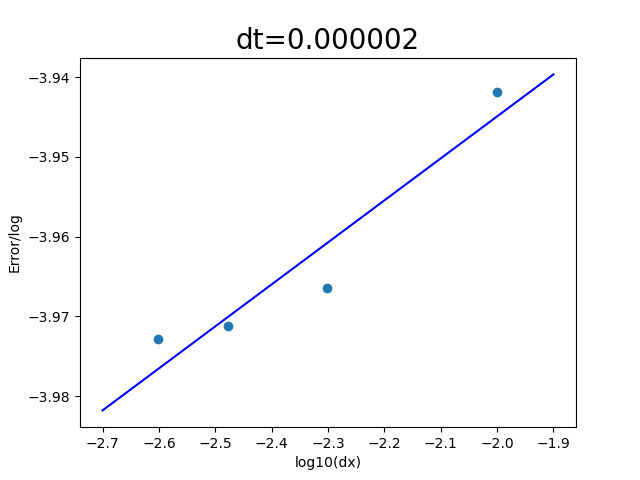
\includegraphics[width=0.48\textwidth]{img/Explicit_alpha.png}}
    \subfigure[beta]{
    \label{fig.sub.2}
    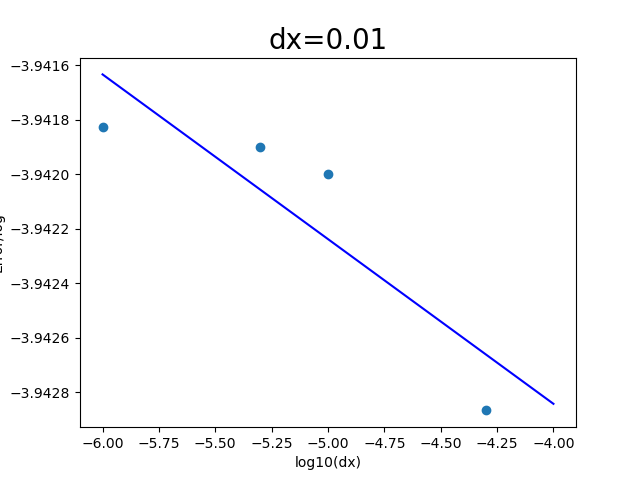
\includegraphics[width=0.48\textwidth]{img/Explicit_beta.png}}
    \caption{Manufactured solution method For Explicit}
    \label{fig:my_label}
\end{figure}

\qquad 得到的$\alpha \approx 0.0526$,$\beta \approx -0.000604$,所以显式格式的误差与网格大小与时间步长关系为:中$e \approx C_1 (\Delta x)^{0.0526} + C_2 (\Delta t)^{-0,000604}$。

\qquad 隐式格式情况下,固定$dt=0.0001$,改变网格数量$n$分别取$100, 200, 300, 400 $得到隐式格式的解,与解析解比较最大误差值$e:=max_{1 \leq i \leq n}\mid u_{exact,i} - u_{num,i}\mid$,对于不同的$\Delta x$得到的不同的误差,得到$\alpha$,同理,固定$dx=0.01$,改变时间步长$dt$分别取$0.01, 0.001, 0.0001, 0.00001$得到不同的解,拟合直线得到关系式中的$\beta$。如下图所示:
\begin{figure}[h]
    \centering
    \subfigure[alpha]{
    \label{fig.sub.1}
    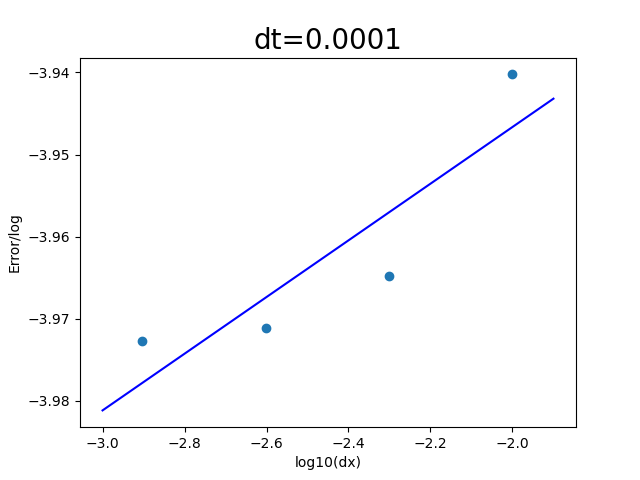
\includegraphics[width=0.48\textwidth]{img/Implicit_alpha.png}}
    \subfigure[beta]{
    \label{fig.sub.2}
    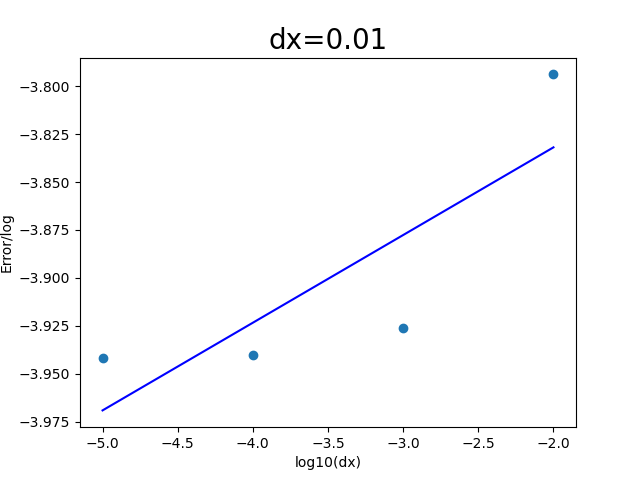
\includegraphics[width=0.48\textwidth]{img/Implicit_beta.png}}
    \caption{Manufactured solution method For Implicit}
    \label{fig:my_label}
\end{figure}

\qquad 得到的$\alpha \approx 0.03452$,$\beta \approx 0.04571$,所以隐式格式关系为:中$e \approx C_1 (\Delta x)^{0.03452} + C_2 (\Delta t)^{0.04571}$。
\subsection{内存检查(Valgrind)}
\qquad 使用valgrind检查内存泄漏情况,结果如图:
\begin{figure}[h]
    \centering
    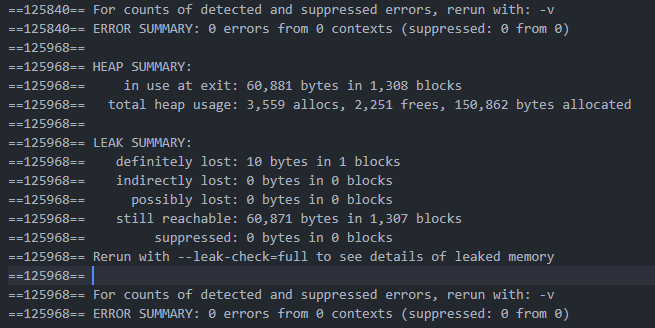
\includegraphics[width=300pt]{img/valgrind.jpg}
    \caption{valgrind结果}
    \label{fig:my_label}
\end{figure}

\qquad 结果中的definitely lost 是由Petsc库中的函数导致的,总体程序并没有错误。
\subsection{隐式格式中不同pc\_type影响}
\qquad 对于$dx=0.01$,$dt=0.00001$的相同条件下,分别使用三种不同的pc\_type,pc\_type为Jacobi时的性能报告如下:
\begin{figure}[h]
    \centering
    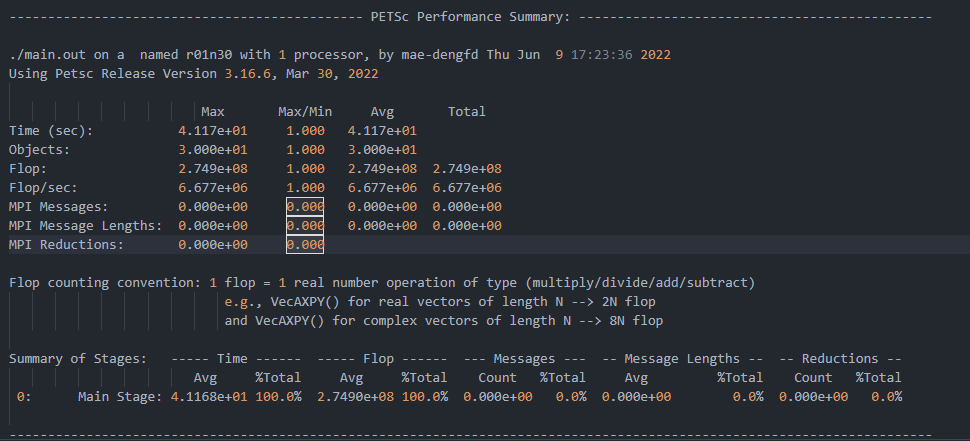
\includegraphics[width=300pt]{img/jacobi.jpg}
    \caption{jacobi}
    \label{fig:my_label}
\end{figure}

\qquad pc\_type为Additive Schwarz时的性能报告如下:
\begin{figure}[h]
    \centering
    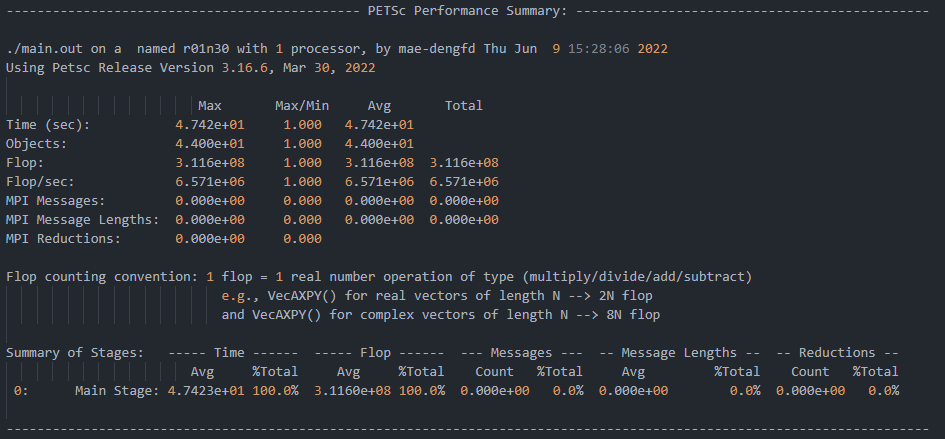
\includegraphics[width=300pt]{img/asm.jpg}
    \caption{Additive Schwarz}
    \label{fig:my_label}
\end{figure}
\clearpage
\qquad pc\_type为LU时的性能报告如下:
\begin{figure}[h]
    \centering
    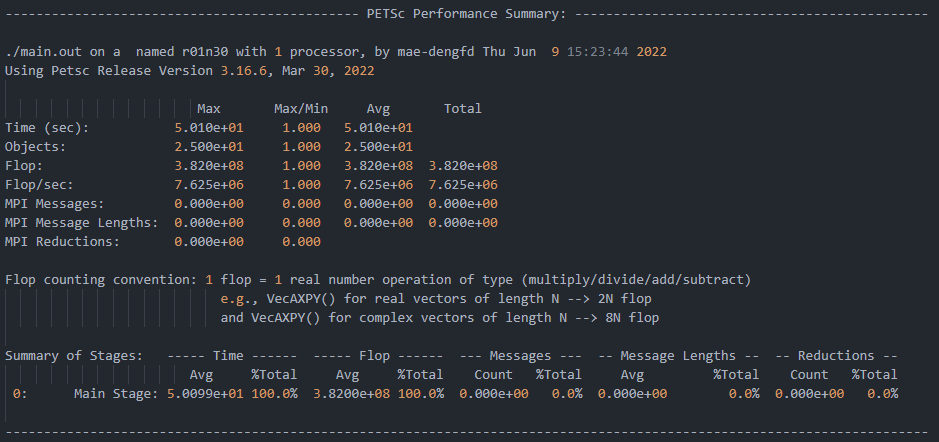
\includegraphics[width=300pt]{img/lu.jpg}
    \caption{LU}
    \label{fig:my_label}
\end{figure}

\qquad 从结果报告中可以得到,对于隐式格式程序Jacobi运行时间最短,asm运行时间最长。

\section{报告总结}
\qquad 本次Project实现了使用显式差分格式和隐式差分格式对一维传热问题的求解,并使用Petsc库对代码做并行化处理,同时借助HDF5库实现最终数值解数据的传输和存储,通过HDF5文件在Petsc中的读写功能实现重启功能防止机器出现突然断电等突发情况。整个过程最终所有的数据可视化图均由python读取HDF5文件绘画制成。
\end{document}
